\documentclass{article}

\usepackage[left=2cm,right=2cm,top=2cm,bottom=2cm]{geometry} 

\usepackage[utf8]{inputenc}   % otra alternativa para los caracteres acentuados y la "ñ"
\usepackage[           spanish % para poder usar el español
                      ,es-tabla % para los captions de las tablas
                       ]{babel}   
\decimalpoint %para usar el punto decimal en vez de coma para los números con decimales

%\usepackage{beton}
%\usepackage[T1]{fontenc}

\usepackage{parskip}
\usepackage{xcolor}

\usepackage{caption}

\usepackage{enumerate} % paquete para poder personalizar fácilmente la apariencia de las listas enumerativas

\usepackage{graphicx} % figuras
\usepackage{subfigure} % subfiguras

\usepackage{amsfonts}
\usepackage{amsmath}

\definecolor{gris}{RGB}{220,220,220}
	
\usepackage{float} % para controlar la situación de los entornos flotantes

\restylefloat{figure}
\restylefloat{table} 
\setlength{\parindent}{0mm}


\usepackage[bookmarks=true,
            bookmarksnumbered=false, % true means bookmarks in 
                                     % left window are numbered
            bookmarksopen=false,     % true means only level 1
                                     % are displayed.
            colorlinks=true,
            allcolors=blue,
            urlcolor=blue]{hyperref}
\definecolor{webblue}{rgb}{0, 0, 0.5}  % less intense blue


\title{\Huge SWAP: Preparación de las herramientas\vspace{10mm}}

\author{\huge David Cabezas Berrido \vspace{10mm} \\ 
  \huge dxabezas@correo.ugr.es \vspace{10mm}}

\begin{document}
\maketitle
\tableofcontents
\newpage

\section{Objetivos}

El objetivo de esta primera práctica es la puesta en marcha de dos máquinas virtuales idénticas que puedan conectarse a internet y entre sí.
Así como la instalación y configuración de ciertos servicios y herramientas, como son Apache, PHP, MySQL, SSH o CURL.

\section{Creación de las máquinas e instalación del sistema}

Comenzamos creando dos máquinas virtuales idénticas, seleccionamos Ubuntu-64b y la configuración recomendada (1 core, 1GB de RAM y 10GB de disco dinámicos).

Ambas máquinas vienen con un adaptador de red NAT por defecto, añadimos un segundo adaptador de red Host-only para que las máquinas puedan comunicarse entre sí. Si no tenemos ninguno, lo podemos crear en \texttt{File -> \ Host Network Manager -> \ Create}.

\begin{figure}[H]
	\centering
	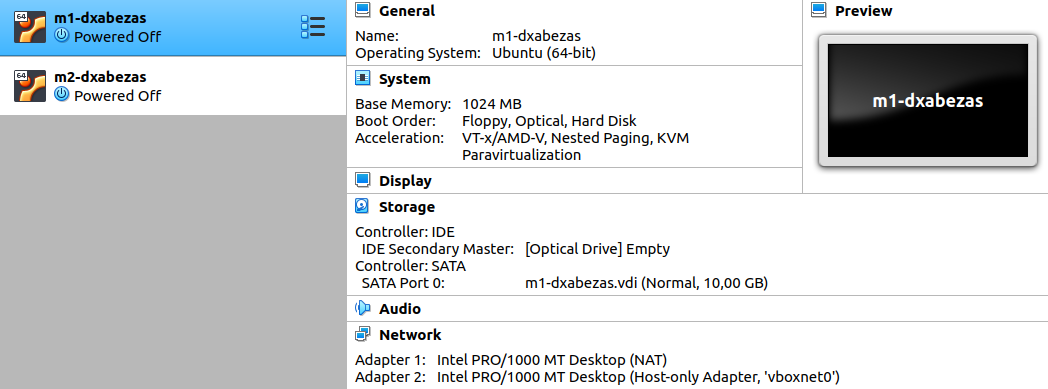
\includegraphics[width=160mm]{imgs/maquinas}
	\caption{Resumen de la configuración de la máquina M1. Observamos que tiene los dos adaptadores de red que hemos comentado.}
	\label{fig:maquinas}
\end{figure}

Seguidamente, instalamos Ubuntu Server 18.04 LTS en ambas máquinas. Podemos descargar la ISO de la página oficial. Creamos en las dos máquinas perfiles idénticos, con usuario \textbf{dxabezas} y constraseña \textbf{Swap1234}.

\begin{figure}[H]
	\centering
	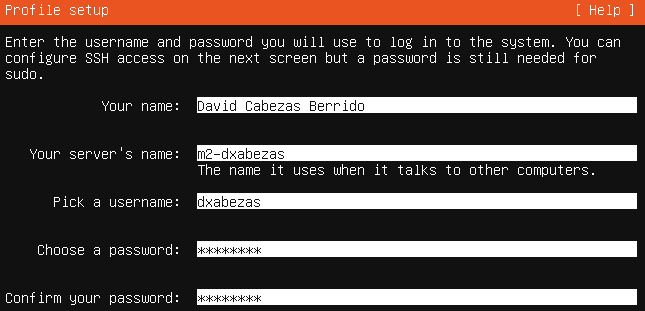
\includegraphics[width=160mm]{imgs/perfil}
	\caption{Creando el perfil en la máquina M2.}
	\label{fig:perfil}
\end{figure}

Durante la instalación escogemos siempre las opciones recomendadas, con la excepción de instalar OpenSSH.

\section{SSH}

Ya tenemos OpenSSH instalado en ambas máquinas. Si durante la instalación no lo hubiésemos marcado, tendríamos que ejecutar:

\begin{verbatim}
	sudo apt-get install openssh-client
	sudo apt-get install openssh-server
\end{verbatim}

Con \texttt{ifconfig}, podemos ver la dirección IP de cada máquina:

\begin{figure}[H]
	\centering
	\subfigure[Máquina 1.]{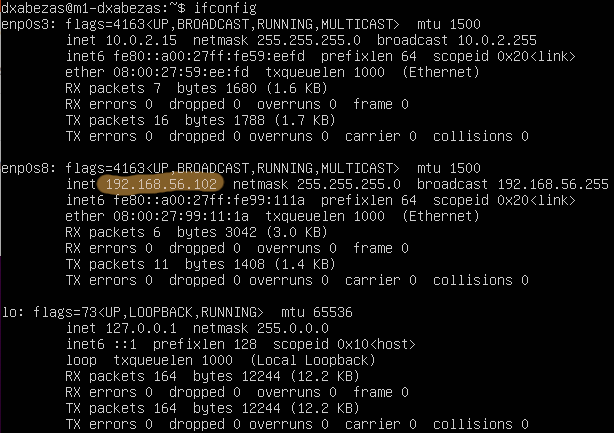
\includegraphics[width=87mm]{imgs/ifconfig1}}
	\subfigure[Máquina 2.]{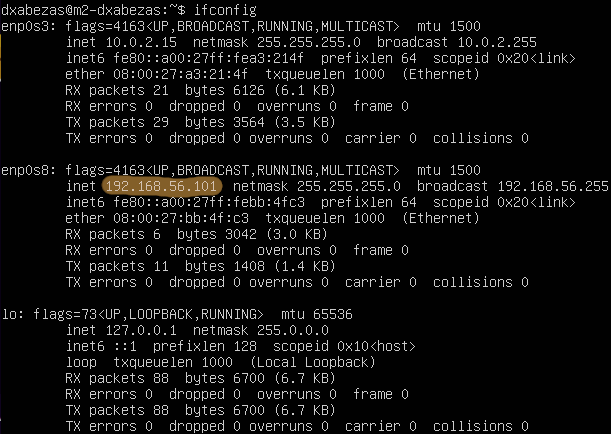
\includegraphics[width=86.5mm]{imgs/ifconfig2}}
	\caption{Direcciones IP de ambas máquinas.}
	\label{fig:ifconfig}
\end{figure}

Nos conectamos de una máquina a otra, ejecutando \texttt{ssh user@ip}.
\begin{figure}[H]
\centering
\subfigure[M1 se conecta a M2.]{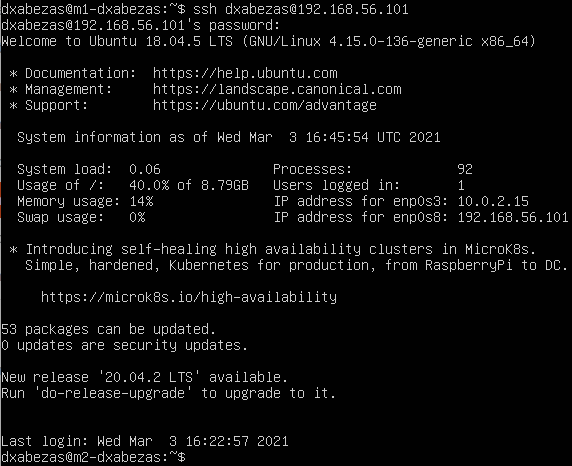
\includegraphics[width=86mm]{imgs/ssh1}}
\subfigure[M2 se conecta a M1.]{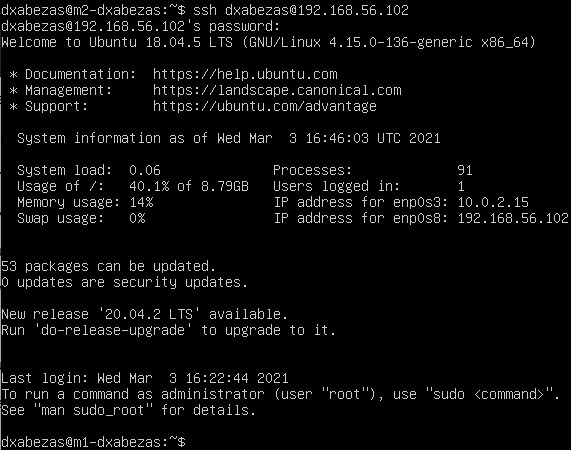
\includegraphics[width=88mm]{imgs/ssh2}}
\caption{Cada máquina se conecta a la otra por SSH con el usuario que creamos (dxabezas, Swap1234).}
\label{fig:ssh}
\end{figure}

\section{Apache2}

Puesto que no marcamos los servicios LAMP durante la instalación, debemos instalarlos manualmente. Empezamos con Apache2, en ambas máquinas ejecutamos:
\begin{verbatim}
	sudo apt install -y apache2
\end{verbatim}

Para comprobar la versión que hemos instalado usamos \texttt{apache2 -v}, y para comprobar que esté en ejecución, 
\begin{verbatim}
	sudo service apache2 status
\end{verbatim}

\begin{figure}[H]
	\centering
	\subfigure[Máquina 1.]{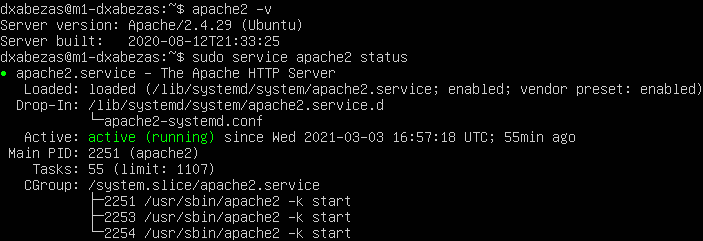
\includegraphics[width=120mm]{imgs/apache1}}
	\subfigure[Máquina 2.]{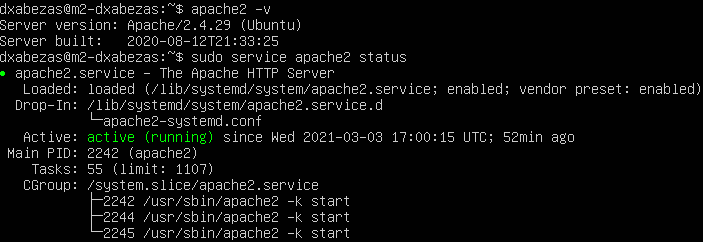
\includegraphics[width=120mm]{imgs/apache2}}
	\caption{Comprobamos la versión de Apache2 y que esté activo.}
	\label{fig:apache2}
\end{figure}



\end{document}